\makeatletter \@ifundefined{rootpath}{\input{../../setup/preamble.tex}}\makeatother
\worksheetstart{Evaluation}{1}{Marts 2, 2015}{Andreas}{../../}
This chapter evaluates \stmnamesp, its associated \ac{STM} library and locking in C\# according to the characteristics defined in \cite[p. 15-21]{dpt907e14trending}. The evaluation will facilitate a conclusion on whether or not language integrated \ac{STM} is a valid alternative to locking as well as discerning whether language integration of \ac{STM} provides any advantages over library based \ac{STM} in terms of usability.
\label{chap:evaluation}
\section{Selected Problems}
As described in \bsref{sec:problem_statement} the evaluation will be conducted by comparing the characteristics of each approach based on a number of concurrent implementations. For this purpose these concurrent problems have been selected:
\begin{enumerate}
\item The dinning philosophers problem\cite[p. 673]{hoare1978communicating}
\item The santa clause problem\cite{trono1994new}
\item A concurrent hashmap implementation\cite[p. 253]{cormen2009introduction}
\end{enumerate}
The dinning philosophers problem represents a well known concurrency problem which highlights some of the pitfalls associated with locking. The santa clause problem encompasses a high degree of modeling as well as requiring complex synchronization. As such, employing this problem helps investigate whether \ac{STM} provides any advantages over locking in such scenarios. Finally a concurrent hashmap implementation represents a real world problem, which benefits from fine grained synchronization and is used in many concurrent implementations. Together these problems provide a varied perspective by exerting different aspects of each approach such as: waiting on one of multiple conditions and fine grained synchronization.

\section{Evaluation Approach}
For each of the selected problem a implementation will be created using, locking, library based \ac{STM} and language based \ac{STM}. Based on these implementations each concurrency approach will be evaluated according to the characteristic defined in our previous work 
\cite[p. 15-21]{dpt907e14trending}. While each of these characteristic range from one extreme to another, a concurrency approach may not reside at on of these extreme, but more likely somewhere in between. Therefore, as part of the evaluation, each concurrency approach will be given a placement on the spectrum of each characteristic, according to the finding of the evaluation. In order to visualize this placement a scale similar to one presented in \bsref{fig:evel_example} is employed. Here \bscode{X} and \bscode{Y} represent the two extremes of the spectrum while the indicators represent the placement of each of the concurrency approaches on the spectrum. As an example \bscode{X} and \bscode{Y} could be low and high writability, \bsref{fig:evel_example} then shows that each of the concurrency approaches resides more towards the high writability end of the spectrum.
\begin{figure}[ht!]
\centering
\includegraphics[scale=0.5]{\rootpath/worksheets/evaluation/figures/eval_example}
\caption{Example of characteristic evaluation scale}\label{fig:evel_example}
\end{figure}
Giving each concurrency approach a visual placement allows for improved communication of the findings along with the ability to easily compare the placement of each concurrency approach.

\section{Implementations}
To ensure common ground between all implementations of a particular problem, a set of requirements detailing common factors which must be true for all implementations of a particular problem has been created.

The dinning philosophers implementations must encompass:
\begin{itemize}
	\item  two 100 milliseconds thread sleeps. One to exemplify the act of eating as well as one upon completing a attempt to eat exemplifying a waiting period before attempting to eat again.
\end{itemize}

 The dinning philosophers implementations must include
 The implementations in their full length can be found in the appendix.


\section{Evaluation of Characteristics}
\subsection{Implicit or Explicit Concurrency}

\begin{figure}[htbp]
\centering
 \includegraphics[width=0.9\textwidth]{\rootpath/worksheets/evaluation/figures/char_implicit_explicit} 
 \caption{Concurrency approaches on the implicit - explicit concurrency spectrum}
\label{fig:char_implicit_explicit}
\end{figure}

\subsection{Fault Restrictive or Expressive Model}

\begin{figure}[htbp]
\centering
 \includegraphics[width=0.9\textwidth]{\rootpath/worksheets/evaluation/figures/char_fault_expressive} 
 \caption{Concurrency approaches on the fault restrictive - expressive spectrum}
\label{fig:char_fault_expressive}
\end{figure}

\subsection{Pessimistic or Optimistic Model}

\begin{figure}[htbp]
\centering
 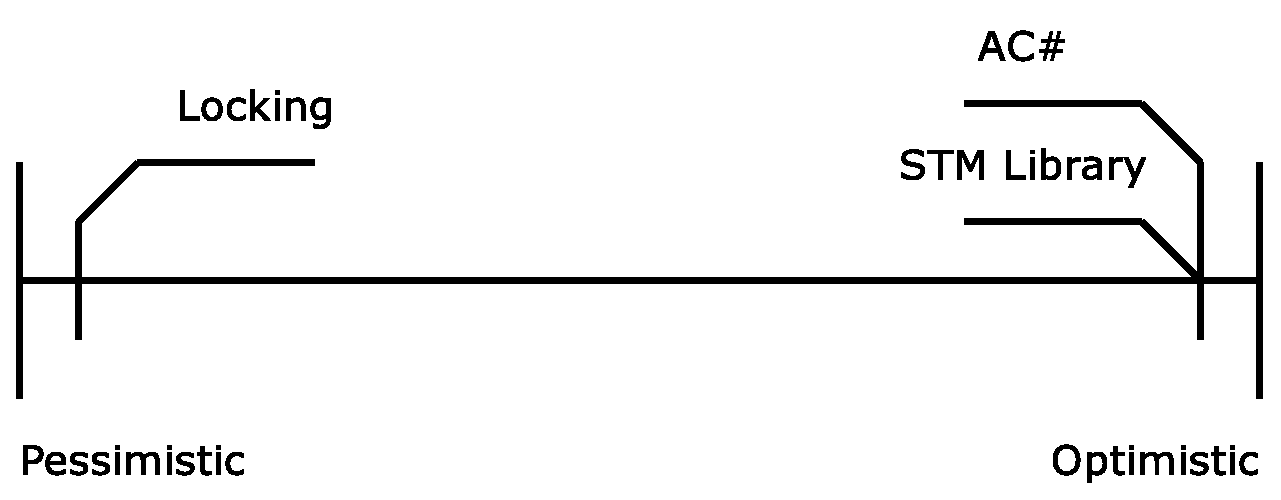
\includegraphics[width=0.9\textwidth]{\rootpath/worksheets/evaluation/figures/char_pessimistic_optemistic} 
 \caption{Concurrency approaches on the pessimistic - optimistic spectrum}
\label{fig:char_pes_opti}
\end{figure}

\subsection{Readability \& Writability}\label{subsec:tl_charac_read_and_write}
As mentioned in \bsref{sec:readability} and \bsref{sec:writablity}, the evaluation of readability and writablity will be based upon the evaluation of the sub characteristics, on which they are based. As two of these, simplicity and orthogonality, are common for both readability and writability, an evaluation of these is presented first. After this, an evaluation of the readability properties of the \ac{TL} concurrency model is presented, followed by the evaluation of \ac{TL} concurrency models level of abstraction and expressivity. Finally an evaluation of the writability of the \ac{TL} concurrency model is presented.
\kasper[inline]{From old report}

%that of simplicity and orthogonality as well as a number of other considerations. Simplicity and orthogonality is described in the following sections followed by a final evaluation of readability.
\subsubsection{Low or High Simplicity}\label{subsec:simplicity}
\begin{figure}[htbp]
\centering
 \includegraphics[width=0.9\textwidth]{\rootpath/worksheets/evaluation/figures/char_read_simplicity} 
 \caption{Concurrency approaches on the low - high simplicity spectrum}
\label{fig:char_simplicity}
\end{figure}

\subsubsection{Low or High Orthogonality}\label{subsec:orthogonality}

\begin{figure}[htbp]
\centering
 \includegraphics[width=0.9\textwidth]{\rootpath/worksheets/evaluation/figures/char_orthogonality} 
 \caption{concurrency approaches on the low - high orthogonality spectrum}
\label{fig:char_orthogonality}
\end{figure}

\subsubsection{Low or High Readability}
\label{subsec:char_readability}

\begin{figure}[htbp]
\centering
 \includegraphics[width=0.9\textwidth]{\rootpath/worksheets/evaluation/figures/char_readability} 
 \caption{Concurrency approaches on the low - high readability spectrum}
\label{fig:char_readability}
\end{figure}

\subsubsection{Low or High Level of Abstraction}\label{subsec:level_of_abstraction}
\begin{figure}[htbp]
\centering
 \includegraphics[width=0.9\textwidth]{\rootpath/worksheets/evaluation/figures/char_level_of_abstraction} 
 \caption{Concurrency approaches on the low - high level of abstraction spectrum}
\label{fig:char_level_of_abstraction}
\end{figure}

\subsubsection{Low or High Expressivity}\label{subsec:expressivity}
\begin{figure}[htbp]
\centering
 \includegraphics[width=0.9\textwidth]{\rootpath/worksheets/evaluation/figures/char_expressivity} 
 \caption{Concurrency approaches on the low - high expressivity spectrum}
\label{fig:char_expressivity}
\end{figure}

\subsubsection{Low or High Writability}
\begin{figure}[htbp]
\centering
 \includegraphics[width=0.9\textwidth]{\rootpath/worksheets/evaluation/figures/char_writability} 
 \caption{Concurrency approaches on the low - high writability spectrum}
\label{fig:char_tl_writability}
\end{figure}

\worksheetend
